\documentclass[12pt]{article}
\usepackage[paper=a4paper,margin=2cm]{geometry}
\usepackage{titling}
\usepackage[colorlinks=true]{hyperref}
\usepackage{enumerate}
\usepackage{amsmath}
\usepackage{enumitem}
\usepackage{graphicx}
\setlength{\parskip}{12pt}
\usepackage{setspace}
\setstretch{1.5}

\setlength{\droptitle}{-6em}

% Enter the specific assignment number and topic of that assignment below, and replace "Your Name" with your actual name.
\title{Term Paper STV2022}
\author{Gard Olav Dietrichson}
\date{\today}

\begin{document}
	\maketitle
	
	\section{Week 1 - Formulate a hypothesis based on existing theories}
	The literature on political representation, and particularly that of women's representation make a distinction between what is known as descriptive and substantive representation (Wangnerud, 2009). While there are other types of representation discussed in political science (Pitkin, 1967), these are the ones that capture most of the active research currently. The distinction between these forms can be summed up as focusing on who legislators \textit{are} and what they \textit{do}. The highly active field is also ripe with the debate on the relation between these two, as some claim that descriptive representation is in fact a necessity in order to ensure substantive represention of minorities' interests (Phillips, 1995).
	
	With my semester task I wish to test whether women representatives in the Norwegian parliament are the central actors that bring about the substantive representation of women, or whether they are simply in line with the party focus. To that end I wish to study the individual speech acts of members of the Norwegian parliament, and discuss how patterns of questions regarding women's issues, and issues that affect women, come about. Who asks these questions? When and Why? And how does the government constellation affect these patterns, given that around 90\% of all questions are asked by opposition politicians?
	
	My central assumption is that women will be more dedicated to holding the government accountable over women's issues. In addition I believe that this tendency could be augmented by party ideology and the responsible minister the question is directed to. 
	
	\section{Find a datasource that could answer the hypothesis}
	Fortunately, these data are easy to find, as the storting has a publicly available API for usage. Even more fortunately, the eminent political scientist Dr. Martin Søyland has created a R-package for easier use of that API. I take advantage of those functions in order to retrieve all the questions that I can get my hands on. However, it should be noted that the API only has data back to 1996, leaving us somewhat wanting in terms of data in the early days of the storting, when a more male dominated storting was present, and women's issues were likely to be viewed with a more consverative bent. However, the data still covers a series of periods coinciding with a different set of government coalitions. It covers 9 different government coalitions, including Jagland, Bondevik I, Stoltenberg I, Bondevik II, Stoltenberg II, Solberg I, Solberg II, Solberg III, and Solberg IV, and Støre I. This includes then several periods of both socialist block government, and socialist block government, and will hopefully help illuminate some of the differences that party and incumbent government can have on MP's furtherance of women's issues in parlimant.
	
	\section{Retrieve and Structure the Data}
	The full documentation for how the data was retrieved can be found in the submitted R-script. But the general outline of this phase of the project can be described as such
	\begin{enumerate}
		\item Collecting data on the sessions and their id numbers
		\item Collecting the meta information on all questions in the sessions
		\item Using this meta data to scrape the actual text of each question
		\item Separately, the relevant MP's for the sessions must be found
		\item When found, their information must be joined with the dataframe containing all the questions.
		\item At this point we have our structured Data.
	\end{enumerate}
	
	The full processes of this can be viewed in the R-script, but a fair warning, some of the scraping procedures take an estimated 14 hours to run. 
	
	\section{Give a brief description of how the data was captured and how they were structured}
	
	The data ended up being a large assortment of questions asked in the Norwegian parliament. In fact, every question asked in the past 26 years is included. It bears mentioning that most of these questions are not relevant to the research question itself, but will be useful in order to construct structural topic modelling, and conduct secondary research into what sort of parliamentarians are most attentive towards women's issues. 
	
	The data is for now structured into rows of individual observations of questions. This means that a single row is an asked question, along with a justification for the question, and a response from the relevant minister. Additionally, there is meta information related to each question, these include type of question, which is important for potential genre differences, as well as personal information in regards to both the question asker, and the person the question is directed to. These variables will later form the basis for our potential regression analysis as part of a set of independent variables. The types of questions can also be used to conduct more in depth analysis in the future, but I wish to use the full dataset to construct my topic model, so I wait with splitting it up. 
	
	There is also a discussion to be had in regards to separating the answer from the question, but given that they are, almost by definition, probably the same topic, I see little reason to do so, but would appreciate feedback on this decision. In addition using the gender of the relevant minister could also be an interesting explanatory variable, to see if women ministers encourage other women to speak up on women's issues relating to that department, such as recently done in Blumenau (2021). I believe that since the topics form the backbone of the analysis, the most important part of the modelling task at hand is to ensure that there is an adequate amount of information that the machine learning model can use to construct a good measure of topics, and the most important influencers of that topic. Both this, and the desire explained in the previous paragraph are reasons for keeping answers and questions together. However, I wish to add another explanation, which is that of genre coherence. The fact remains that all of these questions are from the same forum, namely that of the storting. This means that there is a high likelihood that they share a general language of national politicians, which is connected in time as well as space. Separating the answer, when it structurally might be more similar to the question than it is to an answer formulated to a question on the agenda 20 years ago, might be a source of error, and as such I see even more reason to keep them together.
	
	As for the challenges that I faced in gathering the information, the packages stortingscrape was very useful, and the fact that I have extensive experience using it was also helpful. However, owing to a need to give the storting's database some rest, I made sure to include good manners integer, to set a pause between each scrape. While the database engineers might thank me for that, it also leads to the script requiring 1sec x 51 000 observations to scrape all questions, taking roughly 14-15 hours. 
	
	\section{ Week 2 - Make the necessary pre-processing steps to reduce and standardise your data}
	
	The data used for this week can be found at: \\ https://github.com/Garddi/GardSTV2022H22Repo/blob/main/data/usedata.Rdata 
	
	For this task I chose to pre-process my data in a couple of ways. Given that my stated goal is to run topic modelling on the documents themselves, I need to first tokenize the text, then remove the relevant stopwords, then stem the words, and then finally cast a dfm function that creates a data frame where each document is a row, and each term a column. This dfm is the input of our future LDA model. 
	
	The first step, is to tokenize the text. This splits the text up into singular isolated words, but retains their origin. So that I can, if I so desired, take all the tokens, the individual words, bag all of the ones belonging to the same id and have the complete list of words out again. Tokenizing is the most basic form of splitting a big text up, as it pays no attention to the relationship between words internally in the text given. If you recall my previous hand in, we ended the last program with a dataframe that had a single line for each question, which also came with text explaining the justification for the question, as well as the answer from the relevant minister. All of these variables are relevant when discussing the topic of the question at hand, even the answer, although not spoken by the person bringing the topic up, is still thought to be of the same topic, and related to it. For that reason, before we even tokenize it, I simplify the entire dataset, to only be the text variables, the question type, and the id for the question. This is then used to create a long dataframe of text inputs with attached id. This is then tokenized, split into individual words that make up the texts, this gives us a dataset with 20 600 000 observations, meaning around 20 million tokens in total. Before I limit the words, I find that the average amount of tokens per input is about 400 words. 
	
	The next step is to remove the relevant stopwords. In this instance I choose to use a tf-idf model to select away the most frequent terms across all documents. This model is created through the bind\_tf\_idf function in R. This provides me with a ranked list of the terms appearing based on their tf-idf score, which is a score that calculates how often a term appears across all documents. Meaning the less unique it's appearance is in a document, the lower value it is assigned. After ranking them, I conduct a visual inspection of the terms themselves, and decide on an appropriate cutoff. I find the verb "to secure" which I deem to be possibly relevant to future topic modelling, and decide to use that as a cutoff point, and items with lower tf-idf score than that are listed as "stopwords". I then remove all of those matching words from the complete tokenized list, which leaves me with about 11 200 000 tokens, instead of the 20 million I previously had. I demonstrate the differences in average token amount on the pre and post treated dataframes in the second section. 
	
	Following this, I stem the words using the Quanteda package. This is unfortunately sub-optimal as stemming is a very crude and simplistic method of simplifying words, but it does have it's advantages, namely the low computational requirement, and the uncomplicated implementation. Regardless, in this first draft, I apply a stemming, utilising the Quanteda package. This leads into the final step which is the document feature matrix, created by the cast\_dfm function. 
	
	\section{Visualise the difference between the data before and after the steps taken}
	
	The first comparison I can draw is between zipf's law before and after the treatment. Zipf's law states that the logarithm of the ranking of the appearance of terms, and the logarithm of its' frequency is inversely correlated, meaning these values should fall along a neatly descending line down the scale. The first graph here illustrates this before the treatment
	
	\begin{figure}[h]
		\includegraphics[scale=0.60]{Img/Zipf\_law\_1.PNG}
	\end{figure}
	
	Seen in the first image demonstrating Zipf's law, is that there is a high prevalence of terms that are meaningless when conveying topics. These are usually conjugations, prepositions, and in our case, a sneaky bit of html code is here: br represents the html code for a line break or a paragraph separation, which has avoided the analysis at previous points. This is useful to remove. The next plot then demonstrates this same law, but now with fewer terms
	
	\begin{figure}[h]
		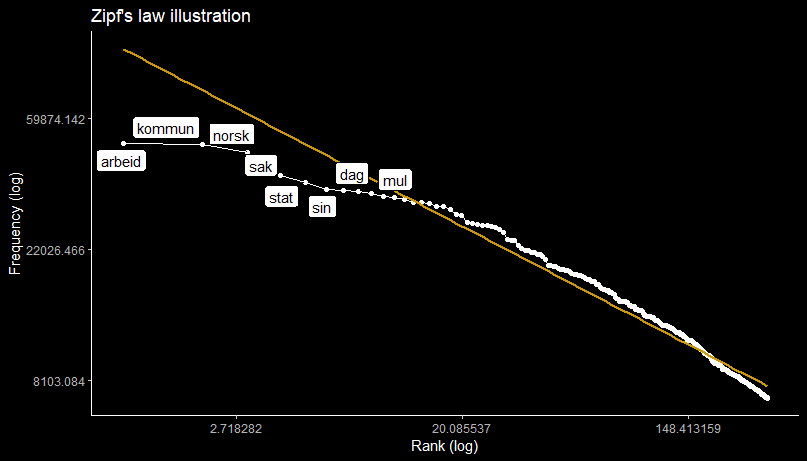
\includegraphics[scale=0.60]{Img/ziplaw2.PNG}
	\end{figure}
	
	This is not quite as neat as was hoped, as some terms do seem more common, and the first 10 or so terms do not fall neatly unto the line itself. However, apart from the initial terms, this line converges more quickly towards the inverse correlation line, and can still be considered and improvement.
	
	The next bit of analysis is in regards to the amount of tokens in each document, following the reductions made. An initial glimpse (code can be found in the script), leads us to realize that there are in fact genre differences between the types of questions, in particular in regards to the lengths of the questions. In relation to this I choose to visualise these separately. 
	
	First there is the interpellations, shown in the first density figure. Demonstrated here is the clear fact that the measures taken has significantly reduced the average tokens per document. As is clear, the peak of the distribution has shifted from above 100 tokens, to below 100 tokens, the squishing that has occured can be explained by the fact that there is probably a lower limit to how many tokens have to be in a text for it to still be meaningful. A text made up of only stopwords is rather pointless.
	
	\begin{figure}[h]
		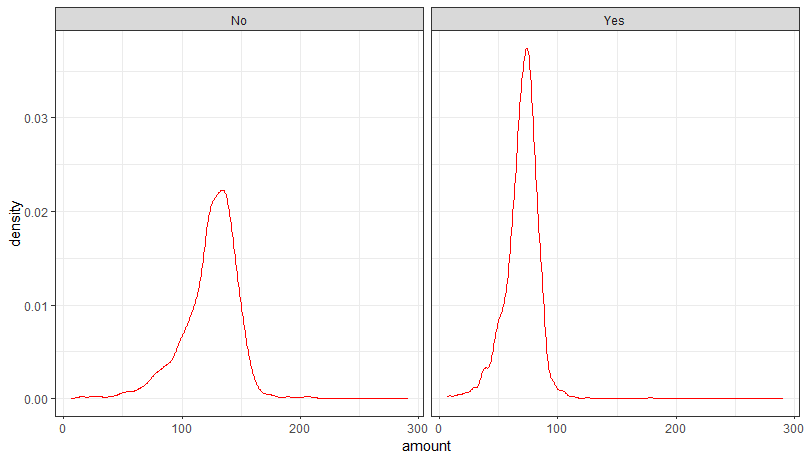
\includegraphics[scale=0.60]{Img/preposttreatedinterpell.png}
	\end{figure}
	
	Next I quickly demonstrate the same pattern for the other cases, the main types of questions, which together make up 99\% of the observations are oral questions, written questions, and question time questions. Note that the "Yes" and "No" graphs note whether they demonstrate the density before or after the removal of stopwords. The lower left graph demonstrates question time questions, and due to the oral nature of these questions, they are considerably shorter than the others. The right figure, demonstrates written questions, and shows the longest potential documents, reaching max values close to 6000 tokens. In between these, we find the oral questions, which are longer than the question time questions. This is again most likely due to genre differences, as question time questions are likely to be more condenced, in an attempt to make them easier to follow for a general audience.
	
	\begin{figure}[h]
		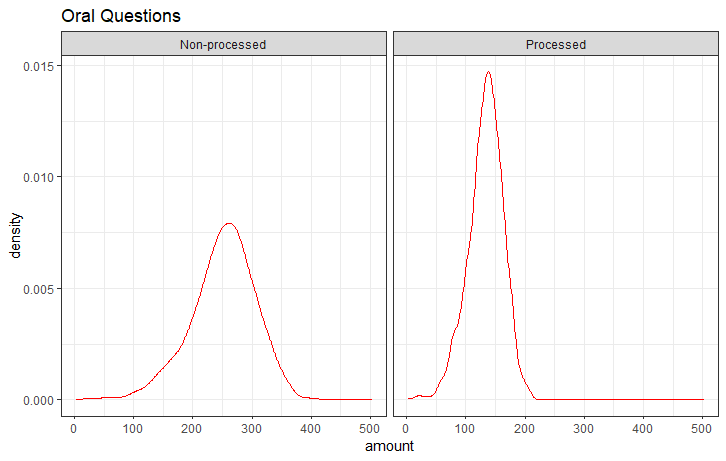
\includegraphics[scale=0.40]{Img/prepostmuntligsporsmal.PNG}
		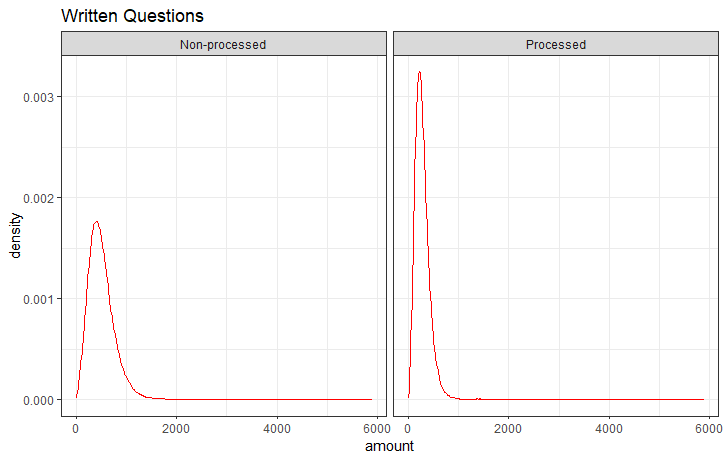
\includegraphics[scale=0.40]{Img/prepostskriftligsporsmal.PNG}
		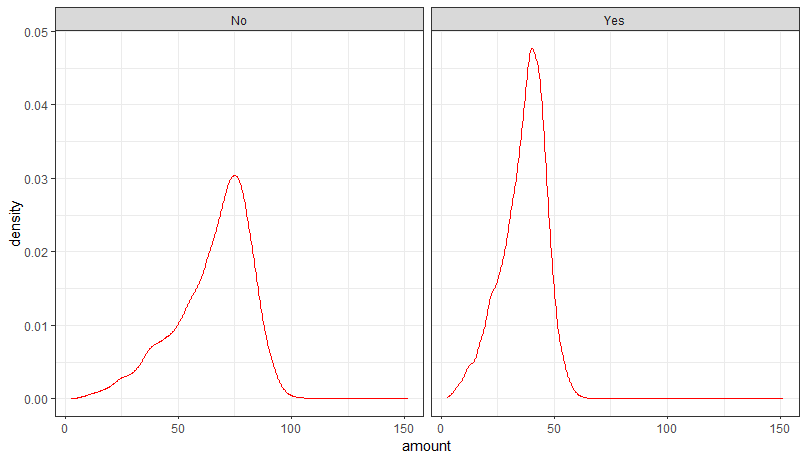
\includegraphics[scale=0.40]{Img/prepostsporretimesporsmal.PNG}
	\end{figure}
	
	
	\section{Discuss the pre-processing critically}
	The pre-processing has not been without its own flaws. I will in this section address issues with both tokenizing, stemming and stopwords. First, tokenizing a text as I have done is most likely the most reductive way of processing a text. The assumption that all words are individual tokens, and their meanings not modified by their neighbours in contexts is highlighted by modifiers often used to convey essential meaning. "Not good" has a clear meaning, but tokenize it and you end up with "Not" and "Good" as separate tokens, and if you apply the bag of words notion, then that meaning can never truly be recovered. However, I maintain that this project does not need to rely on bigrams, given that topic modelling makes little to no assumption about qualifiers, and instead rely on primarily tokens to infer similar meaning. 
	
	The second issue is that of stemming. Stemming is a very simple procedure, as it simply removes what the lexicon identifies as an ending. Two problems become clear, the first is that of verbs that are conjugated irregularly, the second is that of combination words. The understanding of both of these in Norwegian is essential. Irregular conjugation for verbs are verbs that radically change their stem when conjugated in tenses. These verbs are not properly affected by stemming, since removing their ending do not make them into identical tokens to their true infinitive forms. This leads to failure to see two tokens as identical, when they in reality are, and even if there was something to get from keeping them in their proper tenses, the non-similar treatment across all verbs is a practical problem. The second stemming issue has to do with what the lexicon perceives as endings to a word, which are in fact combination words. The most illustrative example is "fastlege" or general practitioner, your general physician. "lege" in this instance is the Norwegian word for physician, however, in New-Norwegian, it is also an ending in a conjugated form of some adverbs. This leads to "fastlege" being stemmed into "fast" which is just the word for permanent, leading to a change in meaning from the word by the act of stemming it. The hope is that the topic model will still recognize the underlying meaning of it, based on its proximity to other relevant words, but it remains an issue. 
	
	Finally there is the issue of stopwords. My method for choosing stopwords may seem arbitrary, and to some degree it is. I encourage scrutiny over the choice of cut-off value in terms of the tf-idf score. 
	
	\section{Week 3 - Identify a strategy for analysing your data}
	
	The goal of this analysis is to investigate a latent grouping of several topics, that are not always directly categorizable, the Storting treats several different cases and topics each year, but they will often be related to an underlying common field of interest, such as women's issues. In order to properly assess the documents and their belonging topic, I have two main choices, a supervised machine learning model, and an unsupervised topic model. I choose the unsupervised topic model for several reasons. First it may be relevant to associate the topic with other topics that I discover during my analysis, if other topics appear in the analysis that could be of interest to my research, then a correlation between these topics might be an interesting find, especially over time. Second there is a time constraint that one needs to be mindful of, and to create a scheme by which I can accurately code a training set would require a lot of theoretical justifications behind it. 
	
	Uniquely, the STM package also allows us to introduce control and effect variables into the topic model, for that reason I will utilise this framework to analyse the interplay between gender and party when focusing on the topics that will be discovered using this model. The dependent variable will be the relative focus that each document affords to issues that I can accurately assess to belong to the category of "women's issues". This process largely draws inspiration from Finseraas et. al. (2021), which utilises the feature of the stm function in order to draw conclusions about the attention given by local MPs to certain topics, following a labour market shock.
	
	\section{Discuss advantages and disadvantages of your strategy}
	
	The advantage of the strategy chosen is that we could potentially receive a rather clear cut answer to the question, by simply looking at the resulting estimated effect that the model spits out. However, even if it is significant, and it turns out that even when controlling for party belonging, that women dedicate a substantially higher focus to what we will be able to accurately assess to be "women's issues" caution should still be exercised. The first issue has to do with the old adage "All models are wrong, but some are useful", a quote sometimes directly attributed to George Box. This quote is even more appropriate when discussing quantitative text analysis. While topic models might functionally be understood as uncovering "topics", what they actually do is concurrent incidents of word pairs, or word groups. Therefore, any analysis should always be critically interpreted, and researchers should be aware of what the model actually says, in addition to the underlying factors it hopefully reflects.
	
	The second issue has to do with the reliability of creating a unified understanding of "women's issues". By its very nature, it is difficult to sort that without having first viewed the data, but when viewed, the topics that are deigned to belong to that overarching meta-topic should be presented and properly argued to belong to the grouping. 
	
	Finally, a potential weakness of this strategy is the potential of failing to uncover the topics themselves. The model would require some fine tunings in order to accurately find all the relevant topics, and there is no guarantee per se, that any amount of tuning will inevitably lead to an accurate isolation of my topics of interest. 
	
	\section{Bibliography}
	
	{\parindent-10pt
		\setstretch{1}
		Blumenau, J. (2019). The Effects of Female Leadership on Women’s Voice in
		Political Debate. \textit{British Journal of Political Science, 51(2), pp. 750-771.} doi:10.1017/S0007123419000334 
		
		Phillips, A. (1995). \textit{The Politics of Presence.} Oxford: Clarendon Press
		
		Pitkin, H. (1967). \textit{The Concept of Representation.} Berkeley: University of California Press
		
		Finseraas, H., Høyland, B. \& Søyland, M. (2021). Climate politics in hard times: How local economic shocks influence MPs attention to climate change. \textit{European Journal of Political Research, 60, pp. 738-747.}
	}
	
\end{document}